
% v2-acmsmall-sample.tex, dated March 6 2012
% This is a sample file for ACM small trim journals
%
% Compilation using 'acmsmall.cls' - version 1.3 (March 2012), Aptara Inc.
% (c) 2010 Association for Computing Machinery (ACM)
%
% Questions/Suggestions/Feedback should be addressed to => "acmtexsupport@aptaracorp.com".
% Users can also go through the FAQs available on the journal's submission webpage.
%
% Steps to compile: latex, bibtex, latex latex
%
% For tracking purposes => this is v1.3 - March 2012
\documentclass[prodmode,acmtecs]{acmsmall} % Aptara syntax
\usepackage[spanish,polish]{babel}
\usepackage[T1]{fontenc}
\usepackage{fancyvrb}
\usepackage{graphicx,hyperref}
\newcommand\cutout[1]{}


\usepackage[table]{xcolor}
\usepackage[utf8]{inputenc}
\usepackage[parfill]{parskip}
\usepackage{tabulary}
\PassOptionsToPackage{hyphens}{url}
\usepackage{hyperref}    
\usepackage[capitalize]{cleveref}


% Metadata Information
% !!! TODO: SET THESE VALUES !!!
\acmVolume{0}
\acmNumber{0}
\acmArticle{CFP}
\acmYear{0}
\acmMonth{0}

\newcounter{colstart}
\setcounter{page}{4}

\RecustomVerbatimCommand{\VerbatimInput}{VerbatimInput}%
{
%fontsize=\footnotesize,
fontfamily=\rmdefault
}


\newcommand{\UnderscoreCommands}{%\do\verbatiminput%
\do\citeNP \do\citeA \do\citeANP \do\citeN \do\shortcite%
\do\shortciteNP \do\shortciteA \do\shortciteANP \do\shortciteN%
\do\citeyear \do\citeyearNP%
}

\usepackage[strings]{underscore}



% Document starts
\begin{document}


\setcounter{colstart}{\thepage}

\acmArticle{CFP}
\title{{\huge\sc SIGLOG Monthly 264}

 August 2025}\author{ELLI ANASTASIADI\affil{Aalborg University, SE}\vspace*{-2.6cm}\begin{flushright}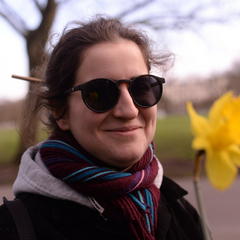
\includegraphics[width=30mm]{elli_anastasiadi.png}\end{flushright}}\begin{abstract}August 2025 edition of SIGLOG Monthly, featuring deadlines, calls and community announcements.
\end{abstract}


\maketitlee

\href{https://lics.siglog.org/newsletters/}{Past Issues}
 - 
\href{https://lics.siglog.org/newsletters/inst.html}{How to submit an announcement}
\section{Table of Contents}\begin{itemize}\item DEADLINES (\cref{deadlines}) 
 
\item CALLS 
 
\begin{itemize}\item SCML (CALL FOR PAPERS) (\cref{SCML})
\item CONFEST 2025 (CALL FOR PARTICIPATION) (\cref{CONFEST2025})
\item ICLP 2025 (CALL FOR PARTICIPATION) (\cref{ICLP2025})
\item Alain Colmerauer Award (CALL FOR NOMINATIONS) (\cref{AlainColmerauerAward})
\end{itemize} 
\item SIGLOG MATTERS 
 
\begin{itemize}\item Message from the SIGLOG Chair (\cref{MessagefromtheSIGLOGChair})
\item CPP 2026 (\cref{CPP2026})
\end{itemize} 
\end{itemize}\section{Deadlines}\label{deadlines}\rowcolors{1}{white}{gray!25}\begin{tabulary}{\linewidth}{LL}Alain Colmerauer Award:  & Aug 19, 2025 (Deadline for s) \\
ICLP 2025:  & Aug 30, 2025 (late registration) \\
CPP 2026:  & Sep 05, 2025 (Abstract Submission Deadline), Sep 12, 2025 (Paper Submission Deadline) \\
FM 2026:  & Nov 25, 2025 (Abstract Submission), Dec 02, 2025 (Full Paper Submission) \\
\end{tabulary}
\section{SCML: A PUBLICATION FORUM FOR SYMBOLIC COMPUTATION AND MACHINE LEARNING}\label{SCML}  An Initiative of the Research Institute for Symbolic Computation (RISC)\\ 
  \href{https://scml.risc.jku.at}{https://scml.risc.jku.at}\\ 
CALL FOR PAPERS 

\begin{itemize}\item  The SCML publishing forum is dedicated to all research that strives to combine Symbolic Computation (SC) and Machine Learning (ML) as two major approaches to ``Artificial Intelligence'', in particular the application of ML to SC, the application of SC to ML, and the hybrid combination of SC and ML to solving problems. We consider submissions that explore the interaction between the two fields - not 
 
  standalone works on either SC or ML.  
 
\item  SCML papers can be continuously submitted and enter the reviewing process immediately after their submission. The final versions of accepted papers are published in the electronic ``RISC Proceedings on Symbolic Computation and Machine Learning''. 
 
\item  Authors of accepted papers are expected to present them at a subsequent SCML workshop. These workshops take place in semi-regular intervals in purely online form (via Zoom), typically in half a day. 
 
\item  Authors of accepted SCML papers that present original research may be invited to submit extended versions of their papers to the SCML Track of the Journal of Symbolic Computation. 
 
\item  Web Page \& Submission: \href{https://scml.risc.jku.at}{https://scml.risc.jku.at} 
 
\end{itemize}\section{Message from the SIGLOG Chair}\label{MessagefromtheSIGLOGChair}MISC 

\begin{itemize}\item  Dear colleagues, 
 
  There is some exciting news about SIGLOG: 
 
  As you may remember from my previous letters, about two years ago ACM decided to increase the overhead charges—i.e., the SIG's annual management fee—and for SIGLOG, the overhead would have risen to 25,000 USD (from the 10,000 USD it had been previously). We could not come up with a viable financial plan to cover this fee, and consequently, we explored the possibility of merging SIGLOG with SIGPLAN. This option, however, was not very popular among our community, as shown by the results of the recent consultation about LICS’s institutional future, promoted by the LICS steering committee. In the same consultation, LICS explored the possibility of becoming an independent conference, which appeared to be a far more popular option. 
 
  This July, the other members of the SIGLOG Executive Committee and I, along with Igor Walukiewicz, the chair of the LICS steering committee, had a meeting with Neha Kumar and Jens Palsberg, the chairs of the SIG Governing Board. We reported the news about the consultation, and in particular, the unwillingness of our community to join SIGPLAN. They explained that we were not alone in this situation; there were other small SIGs that had also been struggling with the overhead increase and were unable to join other SIGs. As a consequence, the SGB started a working group that is planning to revise the overhead formula, with the express goal of helping small SIGs achieve financial stability. They said the current formula was devised to help cover the financial cost of ACM’s transition toward open access. Since institutional support for the new ACM publication model is exceeding expectations, ACM can afford more flexibility toward the SIGs. 
 
  Neha invited the members of the SIGLOG Executive Committee to participate in the working group mentioned above. The goals of this group are not only to revise the SIGs’ overhead formula, but also to rethink the overall SIG structure, and to devise a strategy to cover the publication fees of SIG authors whose institutions do not subscribe to the ACM open access program (authors from subscribing institutions are already covered, of course). We will begin these meetings in August, and hopefully, we will be able to report some good, concrete news soon. Stay tuned! 
 
  I would also like to take this opportunity to express our gratitude to everyone who subscribed to SIGLOG following our appeal several months ago. Your response has been very encouraging—our membership has grown from 185 to around 240. However, the numbers are now declining slowly, probably because older memberships are expiring and some people are not renewing. Hence, I would like to renew our appeal to become a SIGLOG member, or to renew your membership: a strong show of community support is vital as we work with ACM to ensure favorable terms for SIGLOG. 
 
  Catuscia Palamidessi 
 
  Chair of the SIGLOG EC 
 
\end{itemize}\section{CPP 2026:Certified Programs and Proofs}\label{CPP2026}  \href{https://popl26.sigplan.org/home/CPP-2026}{https://popl26.sigplan.org/home/CPP-2026}\\ 
  12-13 January.  Rennes, France\\ 
  co-located with POPL 2026\\ 
CALL FOR PAPERS 

  Certified Programs and Proofs (CPP) is an international conference on practical and theoretical topics in all areas that consider formal verification and certification as an essential paradigm for their work. CPP spans areas of computer science, mathematics, logic, and education.\\ 
  CPP 2026 (\href{https://popl26.sigplan.org/home/CPP-2026}{https://popl26.sigplan.org/home/CPP-2026}) will be held on 12-13 January 2026 and will be co-located with POPL 2026 in Rennes, France. CPP 2026 is sponsored by ACM SIGPLAN, in cooperation with ACM SIGLOG.\\ 
  CPP 2026 will welcome contributions from all members of the community. The CPP 2026 organizers will strive to enable both in-person and remote participation, in cooperation with the POPL 2026 organizers.\\ 
\begin{itemize}\item  NEWS: CPP IS NOW 100% GOLD OPEN ACCESS 
 
 Starting in 2026 all articles published at CPP will be Gold Open Access. Authors should check the Open Access section below for more details on what to expect. 
 
\item  IMPORTANT DATES 
 
\rowcolors{1}{white}{gray!25}\begin{tabulary}{\linewidth}{LL}Abstract Submission Deadline:  & Sep 05, 2025 \\
Paper Submission Deadline:  & Sep 12, 2025 \\
Notification (tentative):  & Nov 13, 2025 \\
Camera Ready Deadline (tentative):  & Dec 01, 2025 \\
Conference:  & Jan 12-13, 2026 \\
\end{tabulary}
 
  Deadlines expire at the end of the day, anywhere on earth. Abstract and submission deadlines are strict and there will be no extensions. 
 
  For more details on the submission instructions please visit the webpage.  
 
\item  ORGANIZERS 
 
\begin{itemize}\item  Kathrin Stark, Heriot-Watt University (conference co-chair)
\item  Yannick Zakowski, ENS Lyon (conference co-chair)
\item  Nikhil Swamy, Microsoft Research (PC co-chair)
\item  Nicolas Tabareau, Inria (PC co-chair)
\end{itemize} 
\item  CONTACT 
 
  For any questions please contact the two PC chairs: 
 
\begin{itemize}\item  Nikhil Swamy nswamy@microsoft.com
\item  Nicolas Tabareau nicolas.tabareau@inria.fr
\end{itemize} 
\end{itemize}\section{CONFEST 2025: CONCUR, FMICS, QEST+FORMATS }\label{CONFEST2025}  \href{https://conferences.au.dk/confest2025/registration}{https://conferences.au.dk/confest2025/registration}\\ 
CALL FOR PARTICIPATION 

\begin{itemize}\item  CONFEST 2025 is an umbrella conference, held from August 25-30, 2025 in Aarhus, Denmark 
 
\begin{itemize}\item  3 main conferences: CONCUR, FMICS, QEST+FORMATS
\item  with 8 invited talks and 75 conference paper presentations
\item  6 co-located workshops: BMQL, EXPRESS/SOS, FMQC, PFQA, RADICAL, SynCoP
\end{itemize} 
  Visit the most happy city in the world! \href{https://happy-city-index.com/Aarhus/}{https://happy-city-index.com/Aarhus/} 
 
  The early registration deadline is unfortunately already past.  
 
\item  Overview 
 
  We are excited to invite you to register for CONFEST 2025, which is an umbrella conference, hosting three major international conferences and six workshops: 
 
\begin{itemize}\item  CONCUR 2025: 36th International Conference on Concurrency Theory
\item  FMICS 2025: 30th International Conference on Formal Methods for Industrial Critical Systems
\item  QEST+FORMATS 2025: Joint International Conference on
\item  Quantitative Evaluation of Systems and
\item  Formal Modeling and Analysis of Timed Systems
\end{itemize} 
\item  These events will take place in Aarhus, Denmark, from August 25 to August 30, offering a fantastic opportunity to follow the latest advancements, and network with researchers and practitioners in these fields. For more information about the conferences and the venue, please visit: \href{https://conferences.au.dk/confest2025}{https://conferences.au.dk/confest2025} 
 
\item  Invited Speakers 
 
\begin{itemize}\item  Alessandro Abate, U of Oxford, UK. Title: Neural synthesis for verification and control of stochastic systems - certificates and abstractions
\item  Christel Baier, TU Dresden, Germany. Title: Linear Temporal Logic with Standpoint Modalities
\item  Lu Feng, University of Virginia, USA. Title: Runtime Safety for Learning-Enabled Cyber-Physical Systems: From Predictive Monitoring to Adaptive Shielding
\item  Arnd Hartmanns, U of Twente, NL. Title: Sound and Modest Approaches to Quantitative Model Checking from Sea to Space
\item  Chris Heunen, U of Edinburgh, UK. Title: Towards categorical quantum concurrency theory
\item  Christoph Matheja, U of Oldenburg, Germany and DTU Denmark. Title: Automating Proof Rules for Probabilistic Programs
\item  Ina Schieferdecker, Independent Researcher, Germany. Title: Empowering Testing with AI - Navigating the growing field of research on AI for software testing
\item  Jiri Srba, Aalborg University, Denmark. Title: On-the-Fly Verification: Advancements in Dependency Graphs
\end{itemize} 
\item Workshops 
 
\begin{itemize}\item  BMQL 2025 - 1st IW on Behavioural Metrics and Quantitative Logics
\item  Express/SOS 2025 - combined IW on Expressiveness in Concurrency and Structural Operational Semantics
\item  FMQC 2025 - IW on Formal Methods in Quantum Computing
\item  PFQA 2025 - Colloquium on Principles of Formal Quantitative Analysis
\item  Radical 2025 -  4th IW on Recent Advances in Concurrency and Logic
\item  SynCoP 2025 - 10th IW on Synthesis of Complex Parameters
\end{itemize} 
  We hope to meet you in Aarhus this summer! CONFEST Organization Committee, Andreas Pavliogannis, Jaco van de Pol 
 
\end{itemize}\section{ICLP 2025: 41st International Conference on Logic Programming (ICLP’25) }\label{ICLP2025}  University of Calabria, Rende, Italy \\ 
  September 12-19, 2025\\ 
  \href{https://iclp25.demacs.unical.it/}{https://iclp25.demacs.unical.it/}\\ 
CALL FOR PARTICIPATION 

\begin{itemize}\item  We are pleased to invite you to participate in the 41st International Conference on Logic Programming (ICLP’25), which will be held at the University of Calabria from September 12-19, 2025. The event will include: 
 
\begin{itemize}\item  4 invited talks (Vladimir Lifschitz, Esra Erdem, Stefania Costantini, and Georg Gottlob)
\item  63 conference paper presentations (24 regular papers and 39 Technical Communications)    
\item  4 Recently Published Research (RPR) presentations
\item  2 co-located events (PPDP 2025 and LOPSTR 2025)
\item  8 workshops
\item  Autumn School
\item  Doctoral Consortium
\item  Logic Programming Contest
\end{itemize} 
\item  Registration is now open.  
 
late registration: Aug 30, 2025 
 
  On-Site Registration is not available. For more information on the registration process, please visit the following webpage: \href{https://iclp25.demacs.unical.it/registration}{https://iclp25.demacs.unical.it/registration} 
 
\item  SCOPE 
 
  Since the first conference In Marseille in 1982, ICLP has been the premier international event for presenting research in logic programming. Contributions span all areas of logic programming, including but not limited to the following: 
 
\begin{itemize}\item  Theoretical Foundations: Formal and operational semantics, Non-monotonic reasoning, Reasoning under uncertainty, Knowledge representation, Semantic issues of combining logic and neural models, Complexity results.
\item  Language Design and Programming Methodologies: Concurrency and parallelism, Mobility, Interacting with ML, Logic-based domain-specific languages, Hybrid logical and imperative/functional languages, Programming techniques, Theory reasoning, Answer set programming, Inductive logic programming, Coinductive logic programming.
\item  Program Analysis and Optimization: Analysis, Transformation, Verification, Debugging, Profiling, Visualization, Logic-based validation of generated programs.
\item  Implementation Methodologies and Applications: Compilation, Constraint implementation, Ethics and trustworthiness, Explainability, Parallel/distributed execution, Search and optimization problems, Heuristic methods, Logic-based prompt engineering, Tabling, User interfaces.
\end{itemize} 
\item  REGISTRATION 
 
  Early fees are available until July 30th AOE, the registration procedure closes August 30th AOE. On-Site Registration is not available. \href{https://iclp25.demacs.unical.it/registration}{https://iclp25.demacs.unical.it/registration} 
 
\item  KEYNOTE SPEAKERS 
 
\begin{itemize}\item  Vladimir Lifschitz, University of Texas at Austin (\href{https://www.cs.utexas.edu/~vl/}{https://www.cs.utexas.edu/~vl/}), September 15
\item  Esra Erdem, Sabanci University (\href{https://people.sabanciuniv.edu/esraerdem/}{https://people.sabanciuniv.edu/esraerdem/}), September 16
\item  Stefania Costantini, University of L’Aquila (\href{https://people.disim.univaq.it/~stefcost/}{https://people.disim.univaq.it/~stefcost/}), September 17
\item  Georg Gottlob, University of Calabria (\href{https://www.unical.it/storage/teachers/georg.gottlob/}{https://www.unical.it/storage/teachers/georg.gottlob/}), September 18
\end{itemize} 
\item  ACCEPTED PAPERS 
 
  The full list of accepted papers is available at the following link: \href{https://iclp25.demacs.unical.it/program/accepted-papers}{https://iclp25.demacs.unical.it/program/accepted-papers} 
 
\item  VENUE  
 
  ICLP’25 will be held on the campus of the University of Calabria in Rende, Italy, during 12-19 September 2025. The University of Calabria is one of Italy's leading academic institutions, renowned for its innovative research and vibrant campus life. Located in the scenic city of Rende, it offers a modern learning environment surrounded by natural beauty and cultural richness. Calabria is a region rich in culture, offering a blend of historical heritage and stunning natural beauty. From its breathtaking coastal spots to its easily accessible mountains, the region provides an unforgettable cultural and culinary experience, savoring authentic dishes made from fresh, local ingredients, such as spicy 'nduja, pasta, potatoes and exquisite desserts. 
 
  For more information about the venue, please visit the following webpage \href{https://iclp25.demacs.unical.it/venue/conference-venue}{https://iclp25.demacs.unical.it/venue/conference-venue}  Useful information about accommodation and travel can be found at the following links: 
 
\begin{itemize}\item  \href{https://iclp25.demacs.unical.it/venue/accommodation}{https://iclp25.demacs.unical.it/venue/accommodation}
\item  \href{https://iclp25.demacs.unical.it/venue/travel-information}{https://iclp25.demacs.unical.it/venue/travel-information}
\end{itemize} 
\item  ORGANIZATION 
 
\begin{itemize}\item  General Chair: Francesco Ricca
\item  Program Co-chairs: Martin Gebser and Daniela Inclezan
\item  Publicity Chairs: Manuel Borroto and Francesco Calimeri
\item  Local Chairs: Antonio Ielo and Giuseppe Mazzotta
\end{itemize} 
\end{itemize}\section{Alain Colmerauer Award: The 2025 edition of the Alain Colmerauer Prize}\label{AlainColmerauerAward}CALL FOR NOMINATIONS 

\begin{itemize}\item  Organized by the Association for Logic Programming 
 
\item  In the summer of 1972, Alain Colmerauer and his team in Marseille developed and implemented the first version of the logic programming language Prolog. Together with both earlier and later collaborations with Robert Kowalski and his colleagues in Edinburgh, this work laid the practical and theoretical foundations for the Prolog and logic programming of today. Prolog and its related technologies soon became key tools of symbolic programming and Artificial Intelligence. 
 
  2022 was celebrated as the Year of Prolog to recognize the 50th anniversary of these events and highlight the continuing significance of Prolog and Logic Programming both for symbolic, explainable AI, and for computing more generally. The celebration inaugurated the ALP Alain Colmerauer Prolog Heritage Prize (in short: the Alain Colmerauer Prize). 2025 marks the fourth awarding of the Alain Colmerauer Prize. 
 
  The Prize is given for recent accomplishments and practical advances in Prolog-inspired computing, understood in a broad sense, where foundational, technological and practical contributions are eligible with proven evidence or potential for the future development of Logic Programming. 
 
\item  The 2025 Award 
 
  Nominations are sought for the 2025 edition of the Alain Colmerauer Prize. 
 
\item  Eligibility 
 
  Any individual or group of individuals can nominate themselves or their institution(s)/organization(s) for the Prize. Nominations should describe work that meets the purpose of the Prize. Submissions that address the well-being of society or of the planet are especially welcome. 
 
\item  Submissions 
 
  Nominations should explain the contribution and argue for its present and future significance. The submissions must not exceed three pages plus references and may optionally be accompanied by up to two letters of support no longer than 500 words each. Submissions should be made by the candidates themselves, in pdf, through EasyChair: \href{https://easychair.org/conferences?conf=acprize2025}{https://easychair.org/conferences?conf=acprize2025} 
 
\item  Selection and award 
 
  The Prize is given for depth, novelty, and proven or potential impact. The winner is selected by the Jury from the submitted nominations in consultation with the Executive Committee of the Association for Logic Programming. Furthermore, a shortlist of up to five finalists may also be selected in the process. The Jury will provide a detailed citation that explains the basis of the awarding of the Prize. 
 
  The winner receives a certificate and cash support of up to 2,000 Euros for attending the conference and award ceremony. If there are multiple winners, this amount is shared. Finalists also receive certificates. 
 
\item  Important dates 
 
\rowcolors{1}{white}{gray!25}\begin{tabulary}{\linewidth}{LL}Deadline for submissions:  & Aug 19, 2025 \\
Notification for shortlist:  & Aug 23, 2025 \\
\end{tabulary}
 
\begin{itemize}\item  Award and presentation of the 2025 Prize: The winner of the 2025 Prize will be announced at the 41st International Conference on Logic Programming (ICLP 2025, Rende, Italy 9-19 September 2025). \href{https://iclp25.demacs.unical.it/}{https://iclp25.demacs.unical.it/}
\end{itemize} 
\item  The 2025 AC Prize Jury 
 
  David S. Warren, Miguel Calejo, Stefania Costantini, Agostino Dovier, Maria Garcia de la Banda, Michael Leuschel 
 
\end{itemize}


\bigskip Links: \href{http://siglog.org/}{SIGLOG website}, \href{https://lics.siglog.org}{LICS website}, \href{https://lics.siglog.org/newsletters/}{SIGLOG Monthly}\end{document}